
\documentclass[fleqn,addpoints]{exam}

\usepackage{amsmath}
\usepackage{graphicx}
\usepackage{cancel}
% \usepackage{polynom}
\usepackage{float}
\usepackage{mdwlist}

% \printanswers

\ifprintanswers
\usepackage{2in1, lscape}
\fi

\title{Math 113 Homework 19}
\author{}
\date{\today}

\begin{document}

\maketitle

\section{From the Book}

\begin{itemize*}
  \item pp. 374-375: 5-8, 15, 25-29, 41, 42, 60
  \item pp. 386-389: 1-4, 14-17, 27, 30, 35, 39, 43-44, 57-58
\end{itemize*}

\ifprintanswers
\section{Pages 374-375}

\begin{description}
\item[5]
$(6, -4)$ and $(9, -7)$
\[
  \sqrt{(-4 - (-7))^2 + (6-9)^2)} = \sqrt{3^2 + 3^2} = \sqrt{18} = 3\sqrt{2}
\]

\item[6]
$(-5, 2)$ and $(-1, 6)$
\[
  \sqrt{(-5 - (-1))^2 + (2-6)^2} = \sqrt{4^2 + (-4)^2} = \sqrt{32} = 4 \sqrt{2}
\]

\item[7]
$(-3, 3)$ and $(0, -3)$
\[
  \sqrt{(-3-0)^2 + (3 - (-3))^2} = \sqrt{(-3)^2 + 6^2} = \sqrt{9 + 36} = \sqrt{45} = 3\sqrt{5}
\]

\item[8]
$(-2, -4)$ and $(4, 0)$
\[
  \sqrt{(-2 - 4)^2 + (-4 - 0)^2} = \sqrt{(-6)^2 + (-4)^2} = \sqrt{52} = 2 \sqrt{13}
\]

\item[15]
We need to compute three distances and verify that they are all equal.  The three line segments are:
\begin{itemize}
  \item $(3, 6)$ to $(7, 12)$: $\sqrt{(7-3)^2 + (12-6)^2} = \sqrt{52} = 2 \sqrt{13}$
  \item $(7, 12)$ to $(11, 18)$: $\sqrt{(11-7)^2 + (18-12)^2} = \sqrt{52} = 2 \sqrt{13}$
  \item $(11, 18)$ to $15, 24$:  $\sqrt{(15-11)^2 + (24-18)^2} = \sqrt{52} = 2 \sqrt{13}$
\end{itemize}

\item[25]
$(-2, -4)$ and $(2, -4)$
\[
  m = \frac{-4 - (-4)}{2 - (-2)} = 0
\]

\begin{figure}[H]
  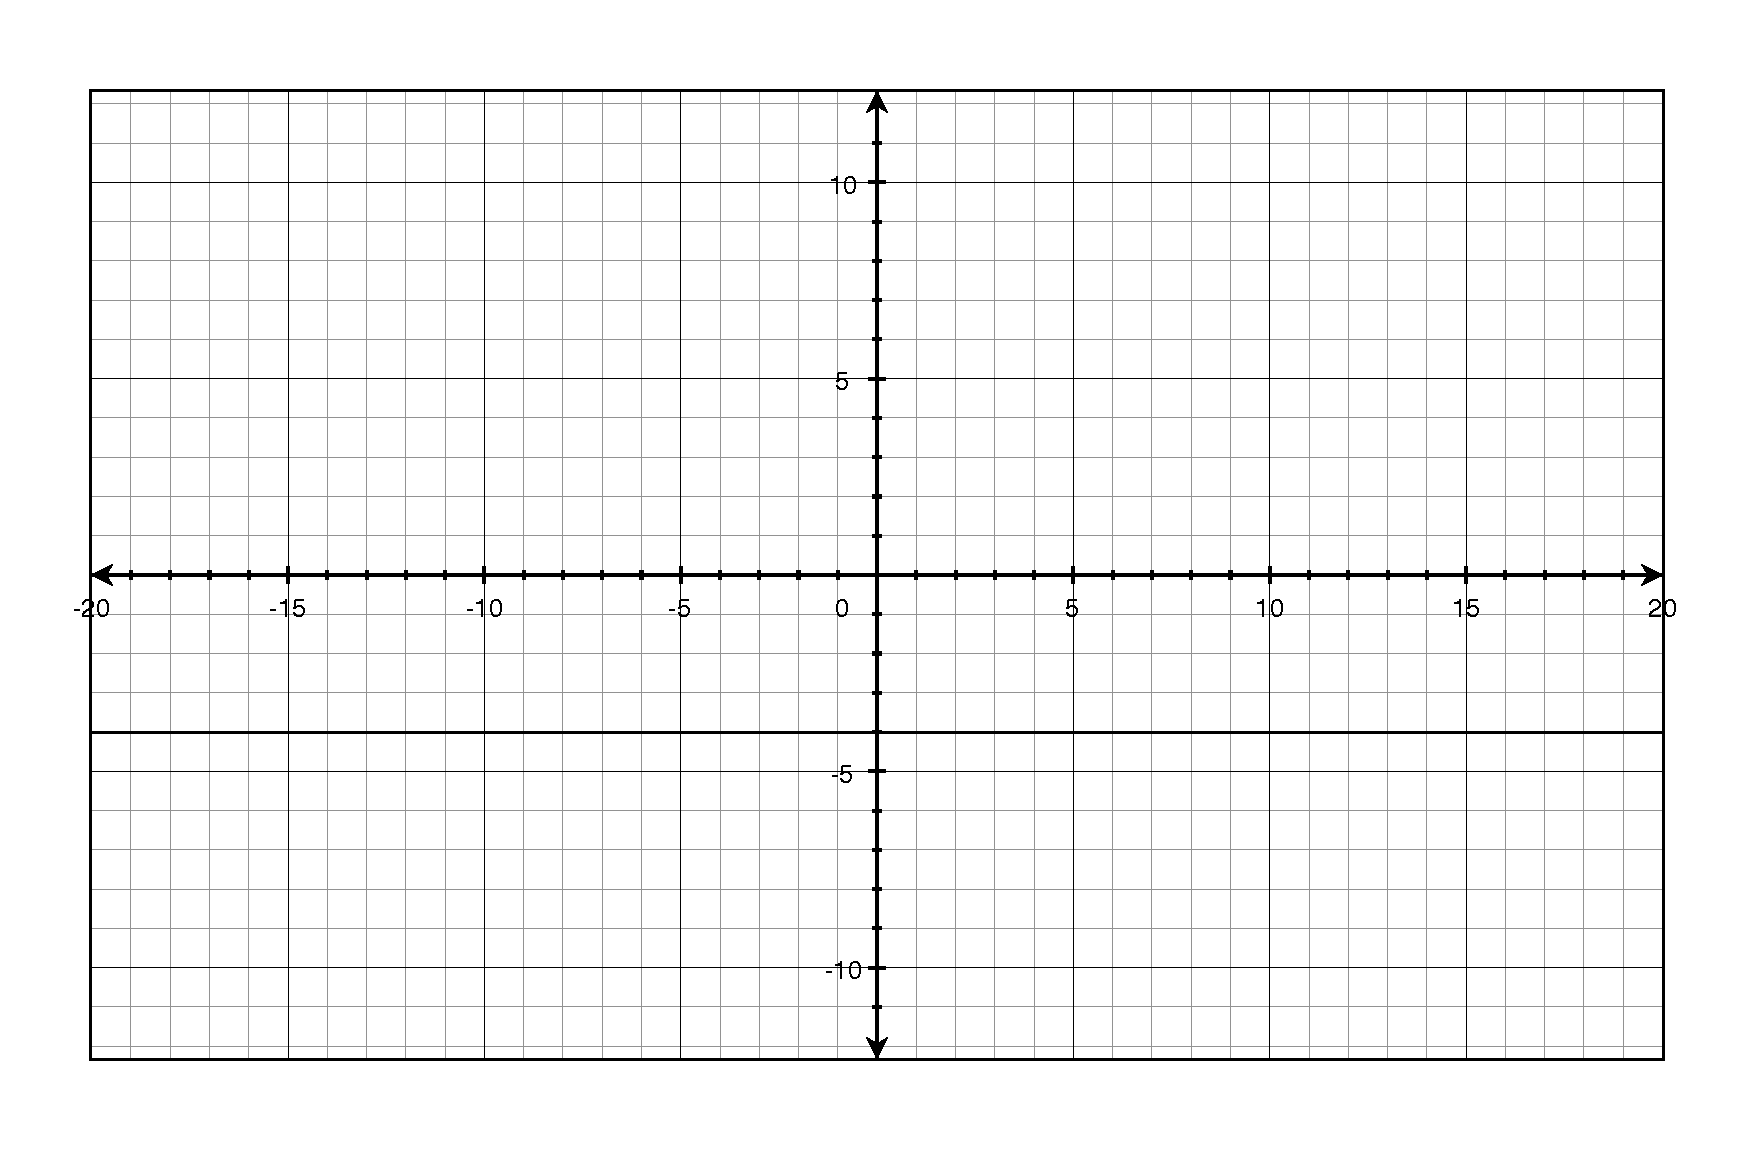
\includegraphics[width=9cm,height=7cm]{p374/25}
\end{figure}

\item[26]
$(1, -5)$ and $(4, -1)$
\[
  m = \frac{-1 - (-5)}{4 - 1} = \frac{4}{3}
\]

\begin{figure}[H]
  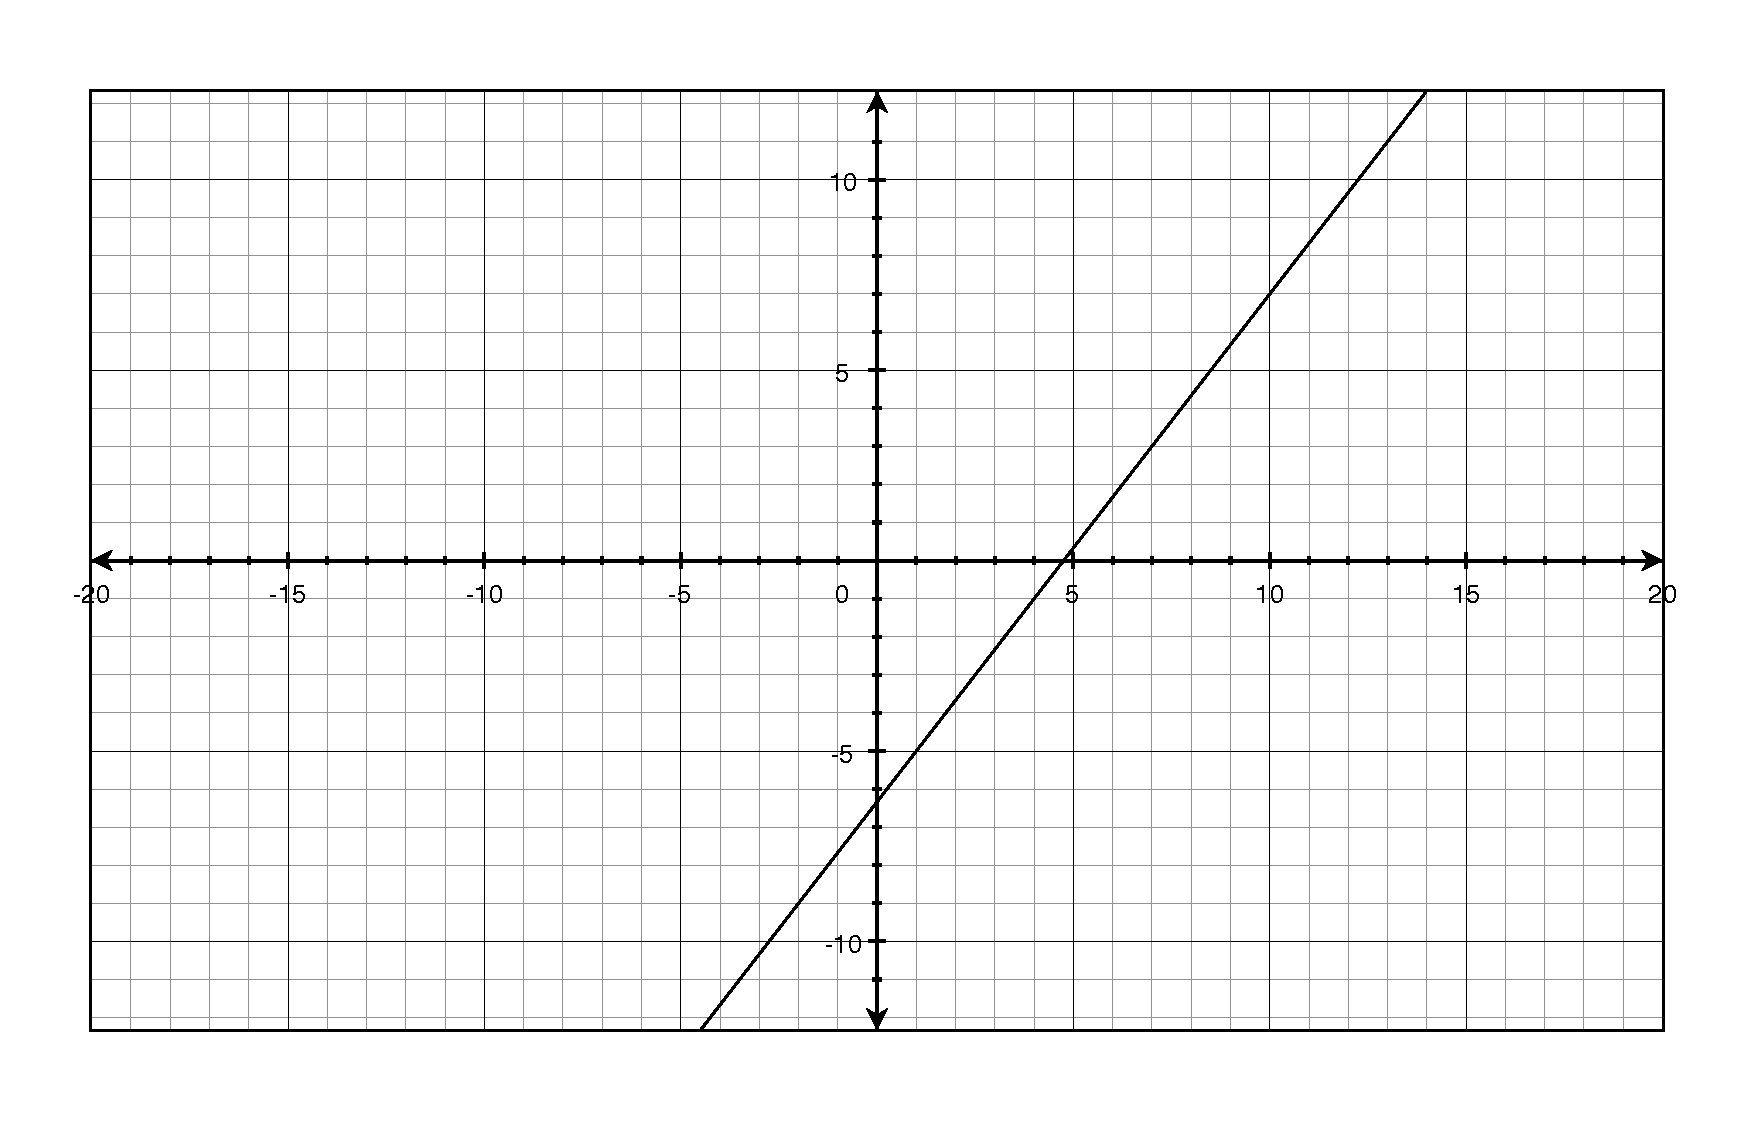
\includegraphics[width=9cm,height=7cm]{p374/26}
\end{figure}


\item[27]
$(0, -2)$ and $(4, 0)$
\[
  m = \frac{0-(-2)}{4-0} = \frac{1}{2}
\]

\begin{figure}[H]
  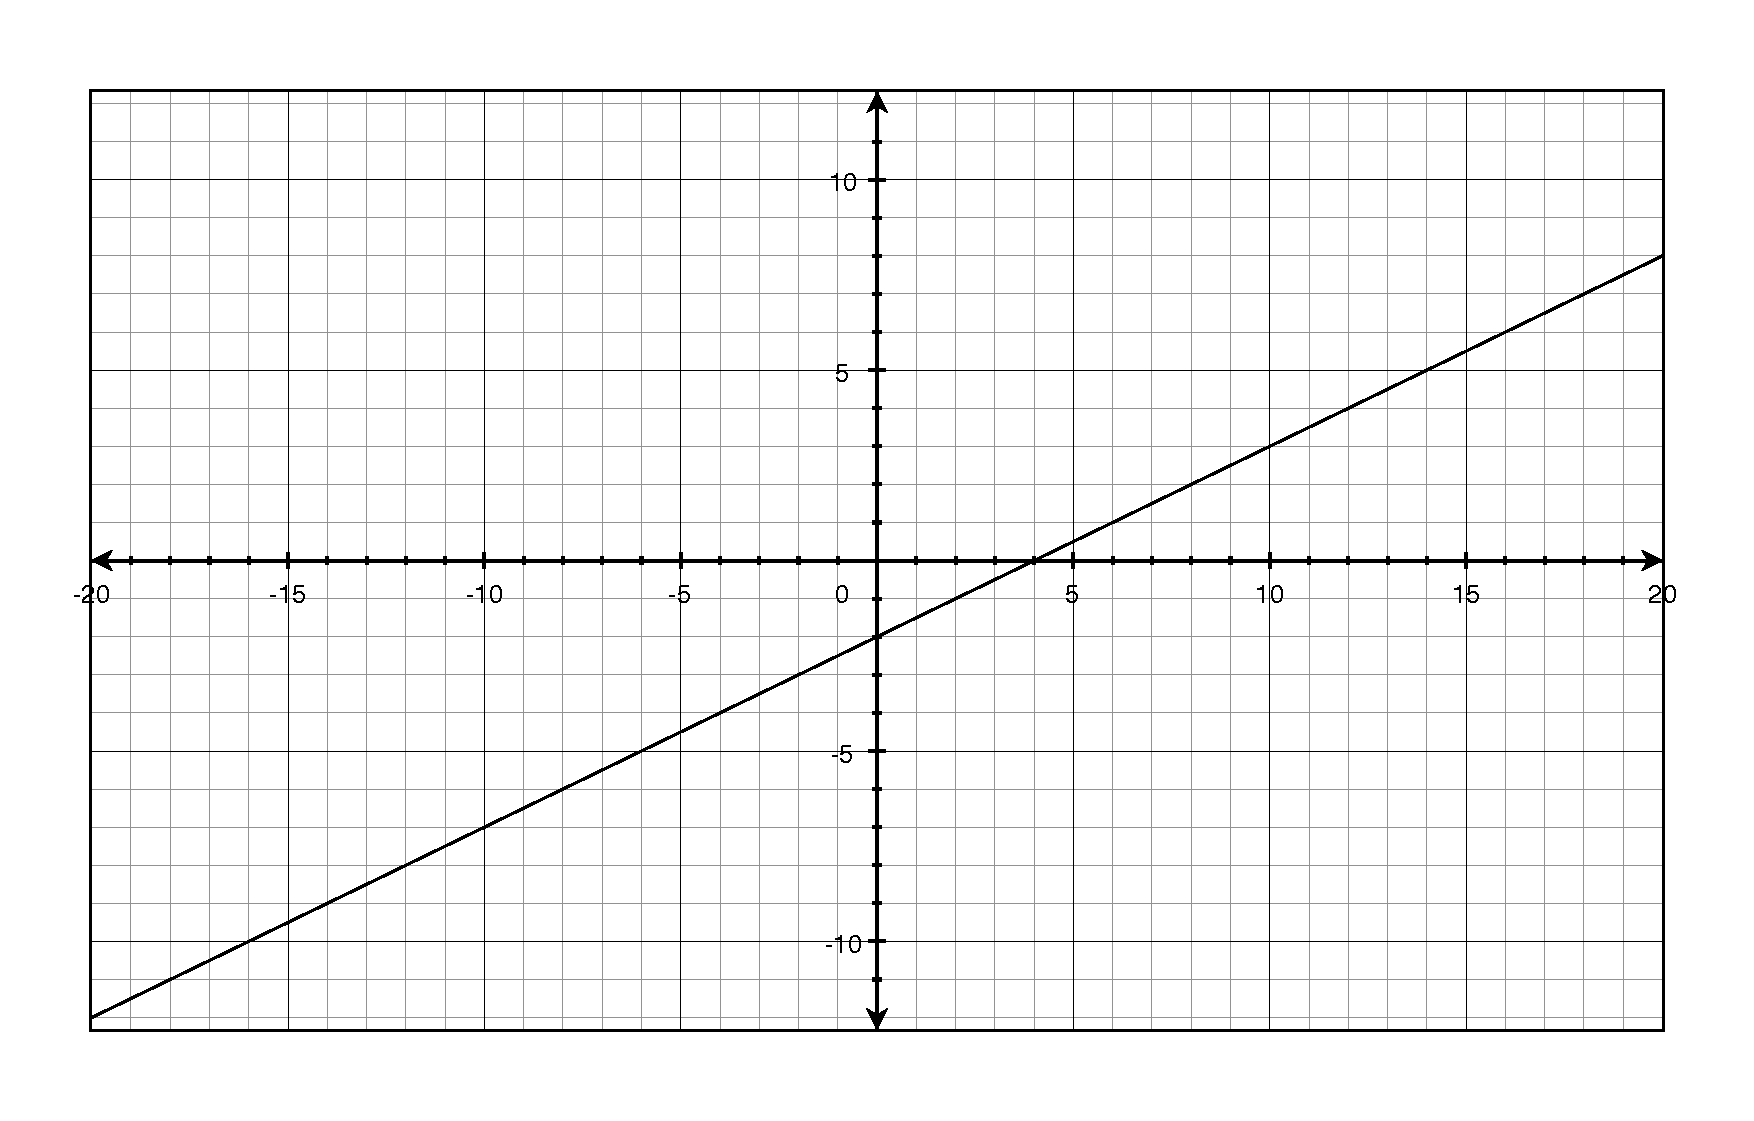
\includegraphics[width=9cm,height=7cm]{p374/27}
\end{figure}

\item[28]
$(-4, 0)$ and $(0, -6)$
\[
  m = \frac{-6-0}{0- (-4)} = - \frac{3}{2}
\]

\begin{figure}[H]
  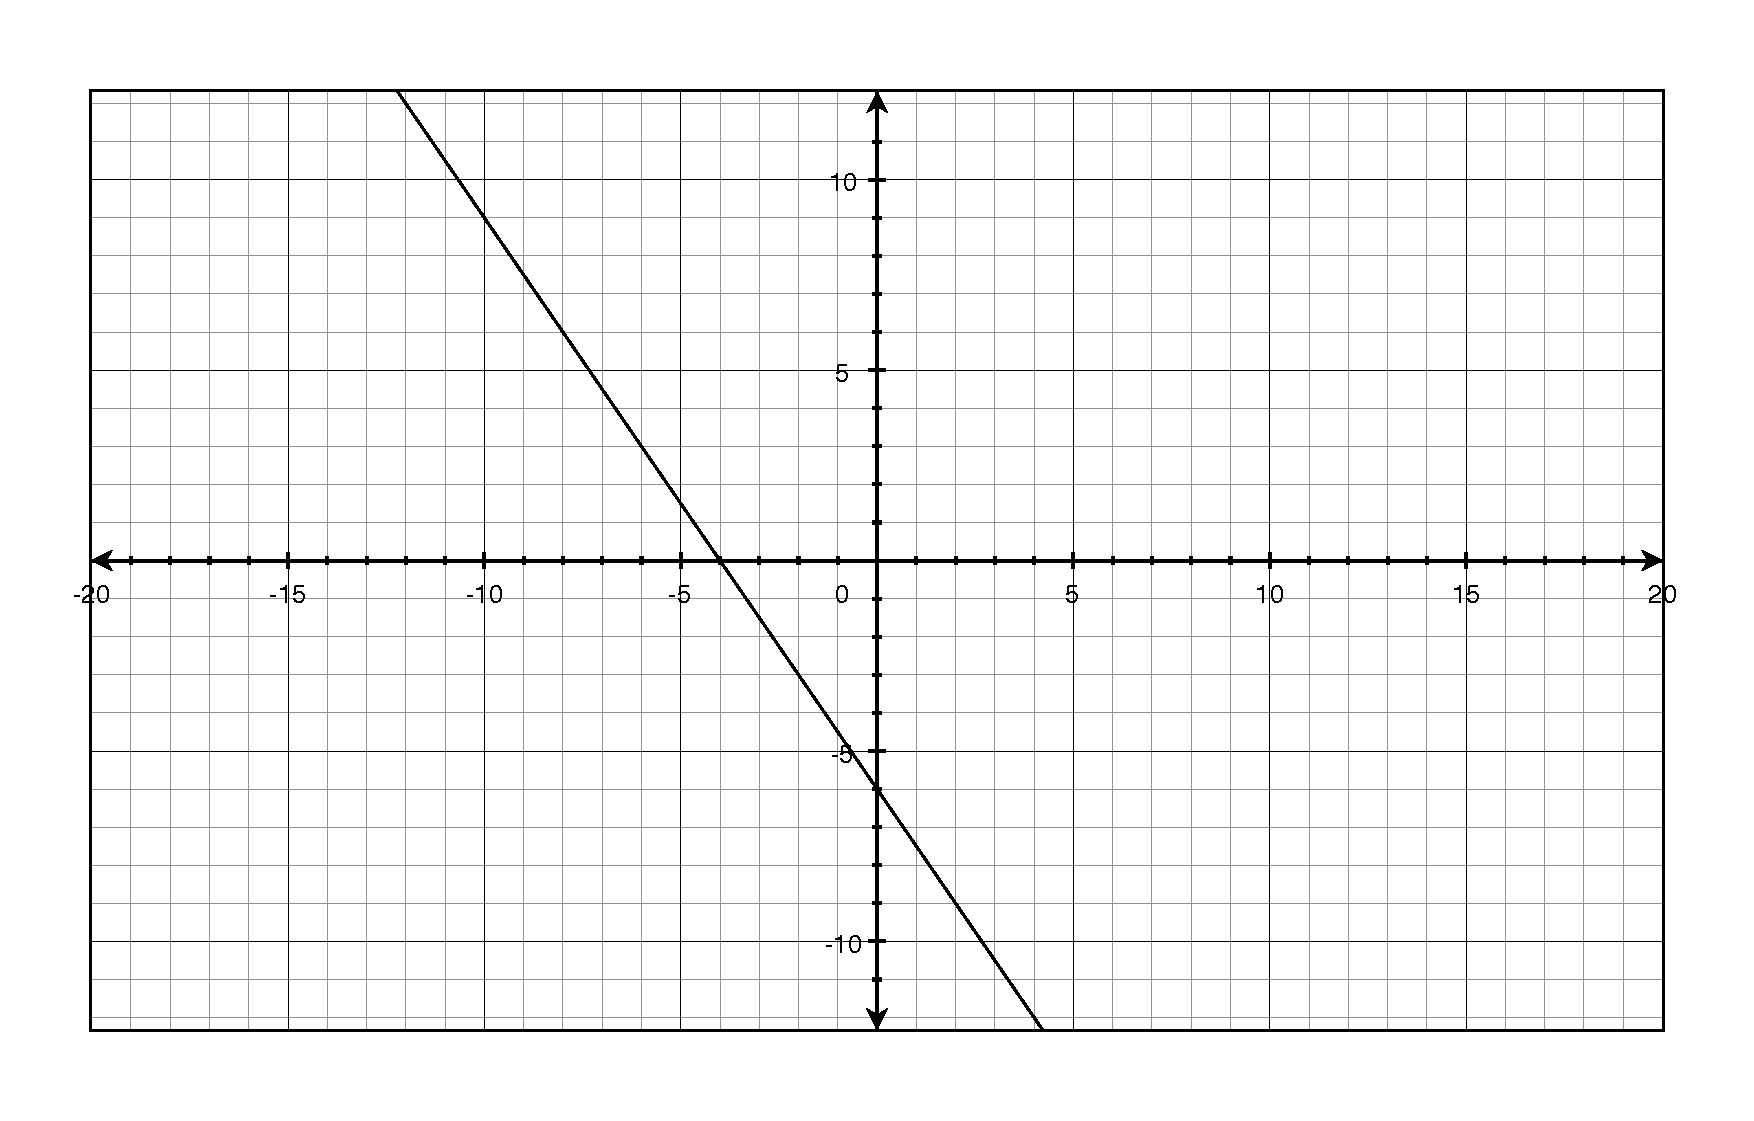
\includegraphics[width=9cm,height=7cm]{p374/28}
\end{figure}


\item[29]
\begin{align*}
  \frac{6-4}{x - (-2)} &= \frac{2}{9} \\
  \frac{2}{x + 2} &= \frac{2}{9} \\
  \frac{1}{x + 2} &= \frac{1}{9} \\
  x+2 &= 9 \\
  x &= 7 \\
\end{align*}

\item[41]
$(3, 1)$ and $m = \dfrac{2}{3}$

\begin{figure}[H]
  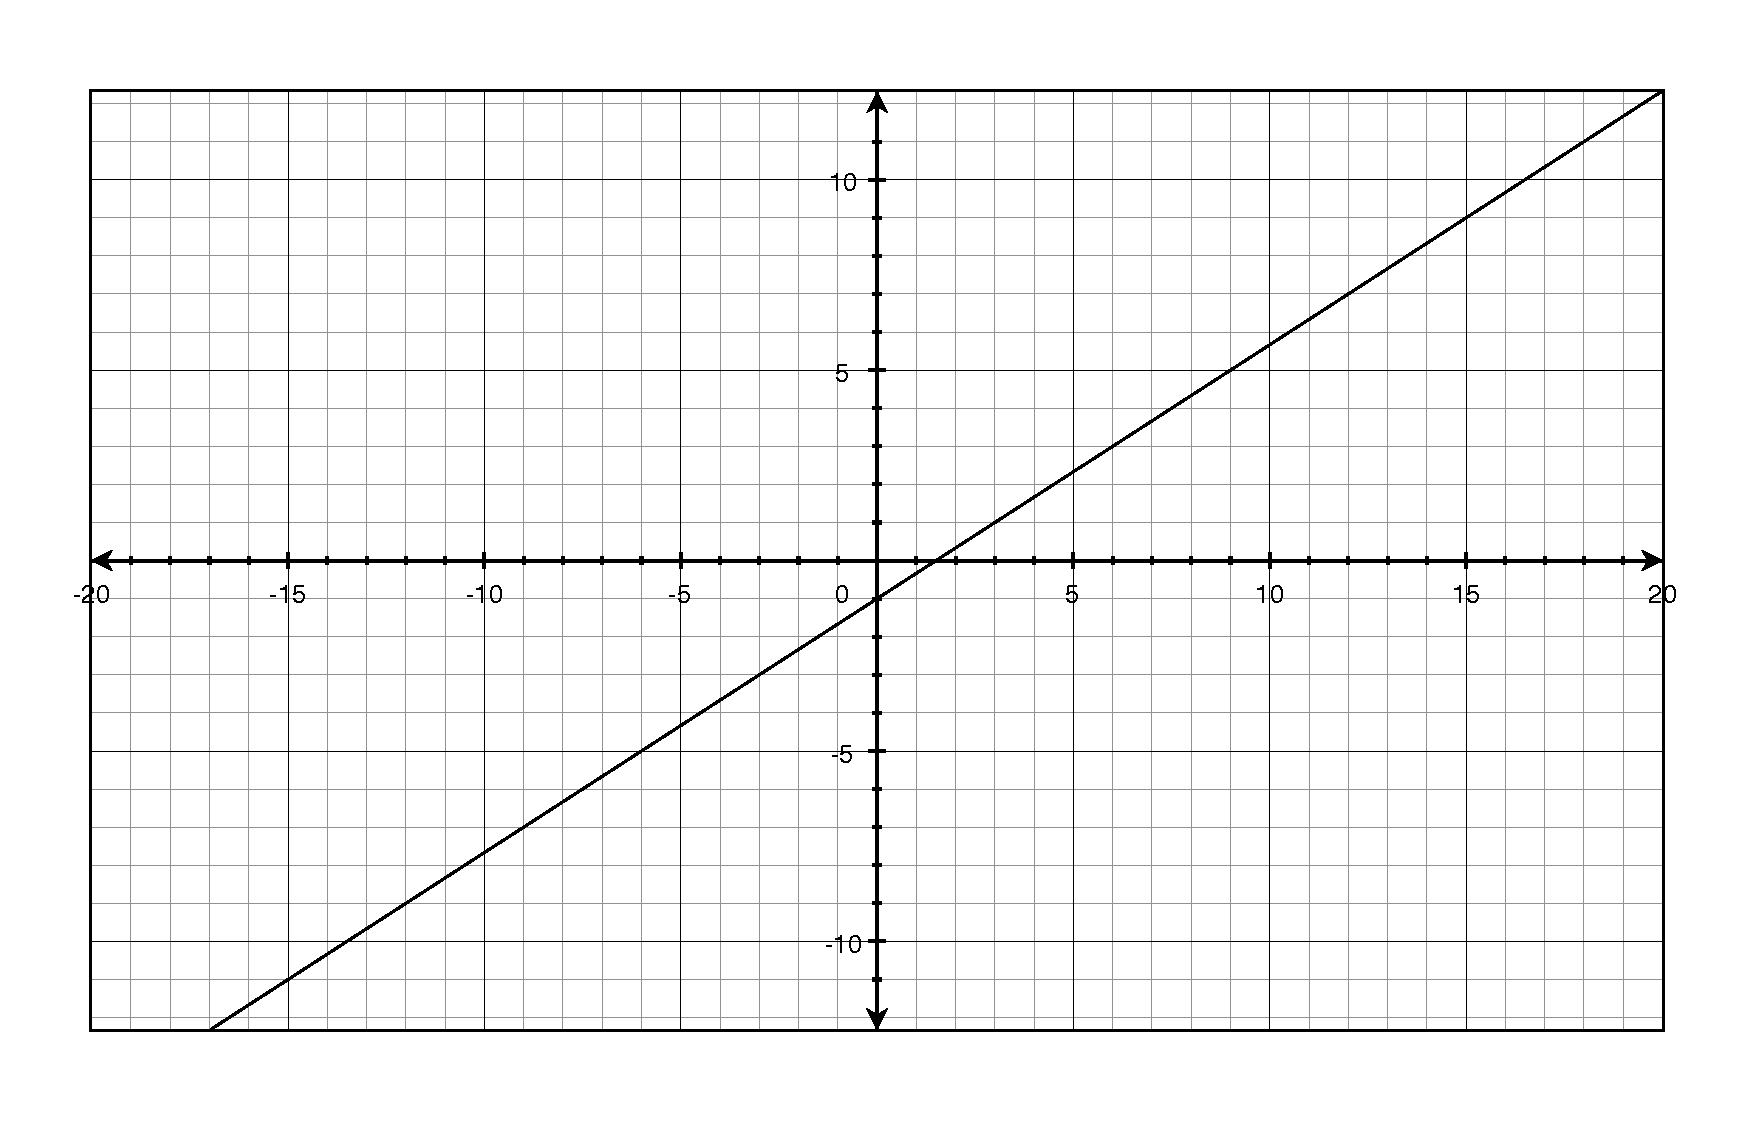
\includegraphics[width=9cm,height=7cm]{p374/41}
\end{figure}


\item[42]
$(-1, 0)$ and $m = \dfrac{3}{4}$

\begin{figure}[H]
  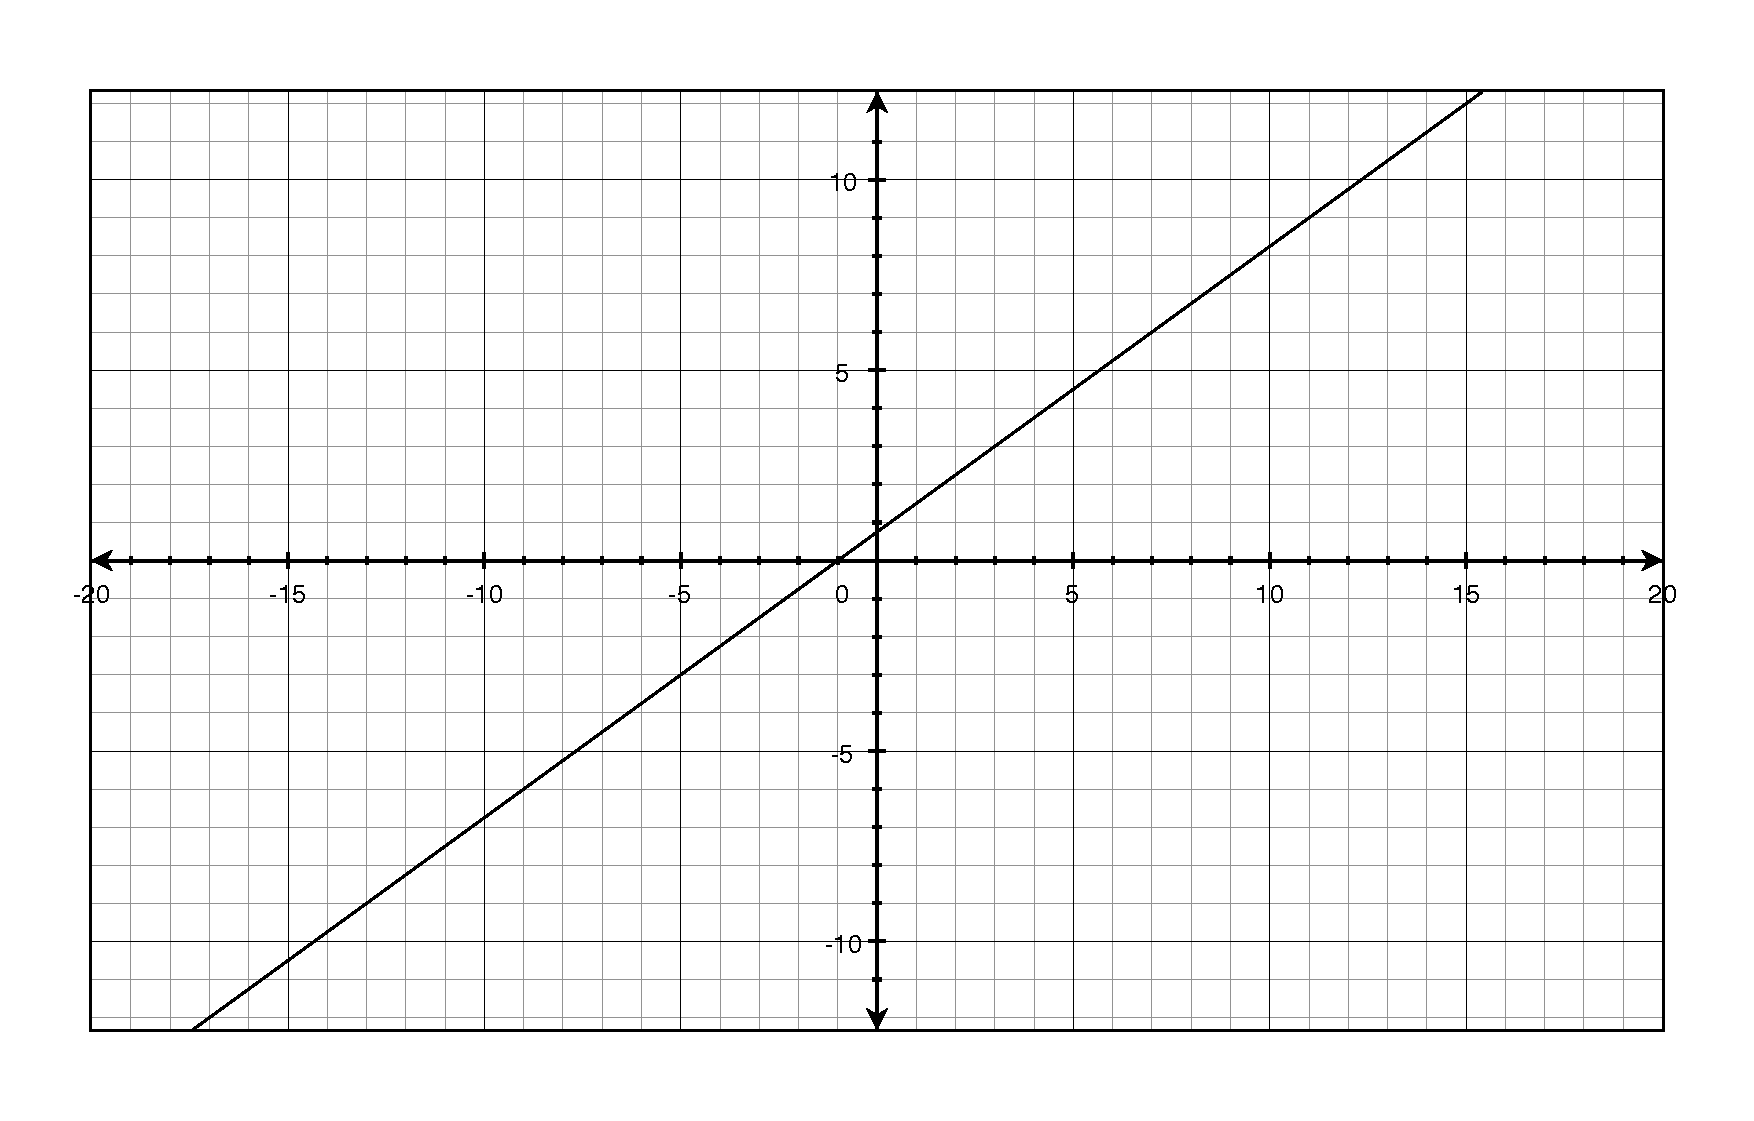
\includegraphics[width=9cm,height=7cm]{p374/42}
\end{figure}

\item[60]
If the grade is 30\%, the road goes up 30 feet in every 100 feet of horizontal distance.  Since the vertical height of
the hill is 75 feet, we can use this ratio to find the change in the horizontal distance:
\begin{align*}
  \frac{30}{100} &= \frac{75}{x} \\
  \frac{3}{10} &= \frac{75}{x} \\
  3x &= 750 \\
  x &= 250 \\
\end{align*}

So the horizontal distance is 250 feet.
 
\end{description}

\section{Pages 374-375}

I computed the equations of the lines using a variety of approaches to show different ways of doing things.  You can use
any approach on any problem.

\begin{description}

\item[1]
$m=\dfrac{1}{2}$ containing $(3, 5)$

\begin{align*}
  y &= \frac{1}{2} x + b \\
  5 &= \frac{1}{2} (3) + b \\
  5 - \frac{3}{2} &= b \\
  b &= \frac{7}{2}
\end{align*}

The equation is:
\begin{itemize}
  \item standard form: $x-2y = -7$
  \item slope/intercept form: $y = \dfrac{1}{2} x + \dfrac{7}{2}$
\end{itemize}

\item[2]
$m = \dfrac{1}{3}$ containing $(2, 3)$

\begin{align*}
  \frac{y-3}{x-2} &= \frac{1}{2} \\
  3(y-3) &= x-2 \\
  3y-9 &= x-2 \\
  3y &= x+7 \\
  y &= \frac{1}{3} x + \frac{7}{3} \\
\end{align*}

\begin{itemize}
  \item standard form: $x-3y=-7$
  \item slope/intercept form: $\dfrac{1}{3} x + \dfrac{7}{3}$
\end{itemize}

\item[3]
$m = 3$ containing $(-2, 4)$

\begin{align*}
  y &= 3x + b \\
  4 &= 3(-2) + b \\
  4 &= -6 + b \\
  b &= 10 \\
\end{align*}

\begin{itemize}
  \item standard form: $3x-y=-10$
  \item slope/intercept form: $y = 3x+10$
\end{itemize}

\item[4]
$m = -2$ containing $(-1, 6)$

\begin{align*}
  \frac{y-6}{x - (-1)} &= -2 \\
  \frac{y-6}{x + 1)} &= -2 \\
  y-6 &= -2(x+1) \\
  y-6 &= -2x - 2 \\
  y &= -2x + 4 \\
\end{align*}

\begin{itemize}
  \item standard form: $2x+y=4$
  \item slope/intercept form: $y = -2x + 4 $
\end{itemize}

\item[14]

$(-2, 5)$ and $(3, -3)$

\[
  m = \frac{5 - (-3)}{-2-3} = - \frac{8}{5}
\]

\begin{align*}
  \frac{y - (-3)}{x-3} &= - \frac{8}{5} \\
  \frac{y + 3}{x-3} &= - \frac{8}{5} \\
  5(y+3) &= -8(x+3) \\
  5y+15 &= -8x+24 \\
  5y &= -8x+9 \\
  y &= - \frac{8}{5} x + \frac{9}{5} \\
\end{align*}

\begin{itemize}
  \item standard form: $8x+5y=9$
  \item slope/intercept form: $y = - \frac{8}{5} x + \frac{9}{5} $
\end{itemize}

\item[15]

$(-1, -4)$ and $(3, -6)$

\[
  m = \frac{-6 - (-4)}{3 - (-1)} = \frac{-6 + 4}{3+1} = - \frac{1}{2}
\]

\begin{align*}
  y &= - \frac{1}{2} x + b \\
  -4 &= - \frac{1}{2} (-1) + b \\
  -4 &= \frac{1}{2} + b \\
  b &= -4 - \frac{1}{2} \\
  b &= - \frac{8}{2} - \frac{1}{2} \\
  b &= - \frac{9}{2} \\
\end{align*}

\begin{itemize}
  \item standard form: $x+2y=-9$
  \item slope/intercept form: $y = - \dfrac{1}{2} x - \dfrac{9}{2}$
\end{itemize}


\item[16]

$(3, 8)$ and $(7, 2)$

\[
  m = \frac{8-2}{3-7} = \frac{6}{-4} = -\frac{3}{2}
\]
\begin{align*}
  \frac{y - 8}{x - 3} &= -\frac{3}{2} \\
  2(y-8) &= -3(x-3) \\
  2y-16 &= -3x+9 \\
  2y &= -3x+25 \\
  y &= - \frac{3}{2} x + \frac{25}{2} \\
\end{align*}

\begin{itemize}
  \item standard form: $3x+2y=25$
  \item slope/intercept form: $y = - \dfrac{3}{2} x + \dfrac{25}{2} $
\end{itemize}

\item[17]

$(0, 0)$ and $(5, 7)$

\[
  m = \frac{7-0}{5-0} = \frac{7}{5}
\]

\begin{align*}
  y &= \frac{7}{5} x + b \\
  0 &= \frac{7}{5} (0) + b \\
  b &= 0 \\
\end{align*}

\begin{itemize}
  \item standard form: $7x-5y=0$
  \item slope/intercept form: $y = \dfrac{7}{5} x$
\end{itemize}

\item[27]

$(2, 0)$ and $(0, -4)$

\[
  m = \frac{0 - (-4)}{2-0} = \frac{4}{2} = 2
\]

\begin{align*}
  \frac{0-y}{2-x} &= 2 \\
  \frac{-y}{2-x} &= 2 \\
  -y &= 2(2-x) \\
  -y &= 4-2x) \\
  y &= 2x-4 \\
\end{align*}

\begin{itemize}
  \item standard form: $2x-y=4$
  \item slope/intercept form: $y = 2x-4 $
\end{itemize}

\item[30]

$(5, 0)$ and $m = -\dfrac{3}{10}$

\begin{align*}
  y &= -\frac{3}{10} x + b \\
  0 &= -\frac{3}{10} (5) + b \\
  0 &= -\frac{3}{2} + b \\
  b &= \frac{3}{2}
\end{align*}

So the equation is: $y = \dfrac{3}{10} x + \dfrac{3}{2}$

\begin{itemize}
  \item standard form: $3x+10y=15$
  \item slope/intercept form: $y = -\dfrac{3}{10} x + \dfrac{3}{2}$
\end{itemize}

\item[35]

Contains $(1, 3)$ and is parallel to $x+5y=9$.

First, we need to find the slope:
\begin{align*}
  x+5y=9 \\
  5y=-x + 9 \\
  y= - \frac{1}{5} x + \frac{9}{5} \\
\end{align*}

So $m = - \dfrac{1}{5}$

Now we can find the equation for a line with this slope which contains $(1, 3)$:
\begin{align*}
  \frac{3-y}{1-x} = - \frac{1}{5} \\
  5(3-y) &= -(1-x) \\
  15-5y &= x-1 \\
  -5y &= x-16 \\
  y &= -\frac{1}{5} x + \frac{16}{5} \\
\end{align*}

\begin{itemize}
  \item standard form: $x+5y=16$
  \item slope/intercept form: $y = -\dfrac{1}{5} x + \dfrac{16}{5} $
\end{itemize}

\item[39]

Contains $(-1, 3)$ and is perpendicular to $2x-y=4$.

First, we need to find the slope of the original line:
\begin{align*}
  2x-y &= 4 \\
  -y &= -2x + 4 \\
  y &= 2x -4 \\
\end{align*}

The slope of the new line is the negative reciprocal of the original slope $m = - \dfrac{1}{2}$

Now we can find the equation for a line with this slope which contains $(-1, 3)$:
\begin{align*}
  y &= - \frac{1}{2} x + b \\
  3 &= - \frac{1}{2} (-1) + b \\
  3 &= \frac{1}{2} + b \\
  b &= 3 - \frac{1}{2} \\
  b &= \frac{6}{2} - \frac{1}{2} \\
  b &= \frac{5}{2} \\
\end{align*}

\begin{itemize}
  \item standard form: $x+2y=5$
  \item slope/intercept form: $y = -\dfrac{1}{2} x + \dfrac{5}{2}$
\end{itemize}

\item[43]

\begin{align*}
  3x+y &= 7 \\
  y &= -3x + 7 \\
\end{align*}

$m = -3$ and $b = 7$

\item[44]

\begin{align*}
  5x - y &= 9 \\
   - y &= -5x + 9 \\
   y &= 5x - 9 \\
\end{align*}

$m=5$ and $b = -9$

\item[57]
$y = - \dfrac{2}{5} x - 1$

\begin{figure}[H]
  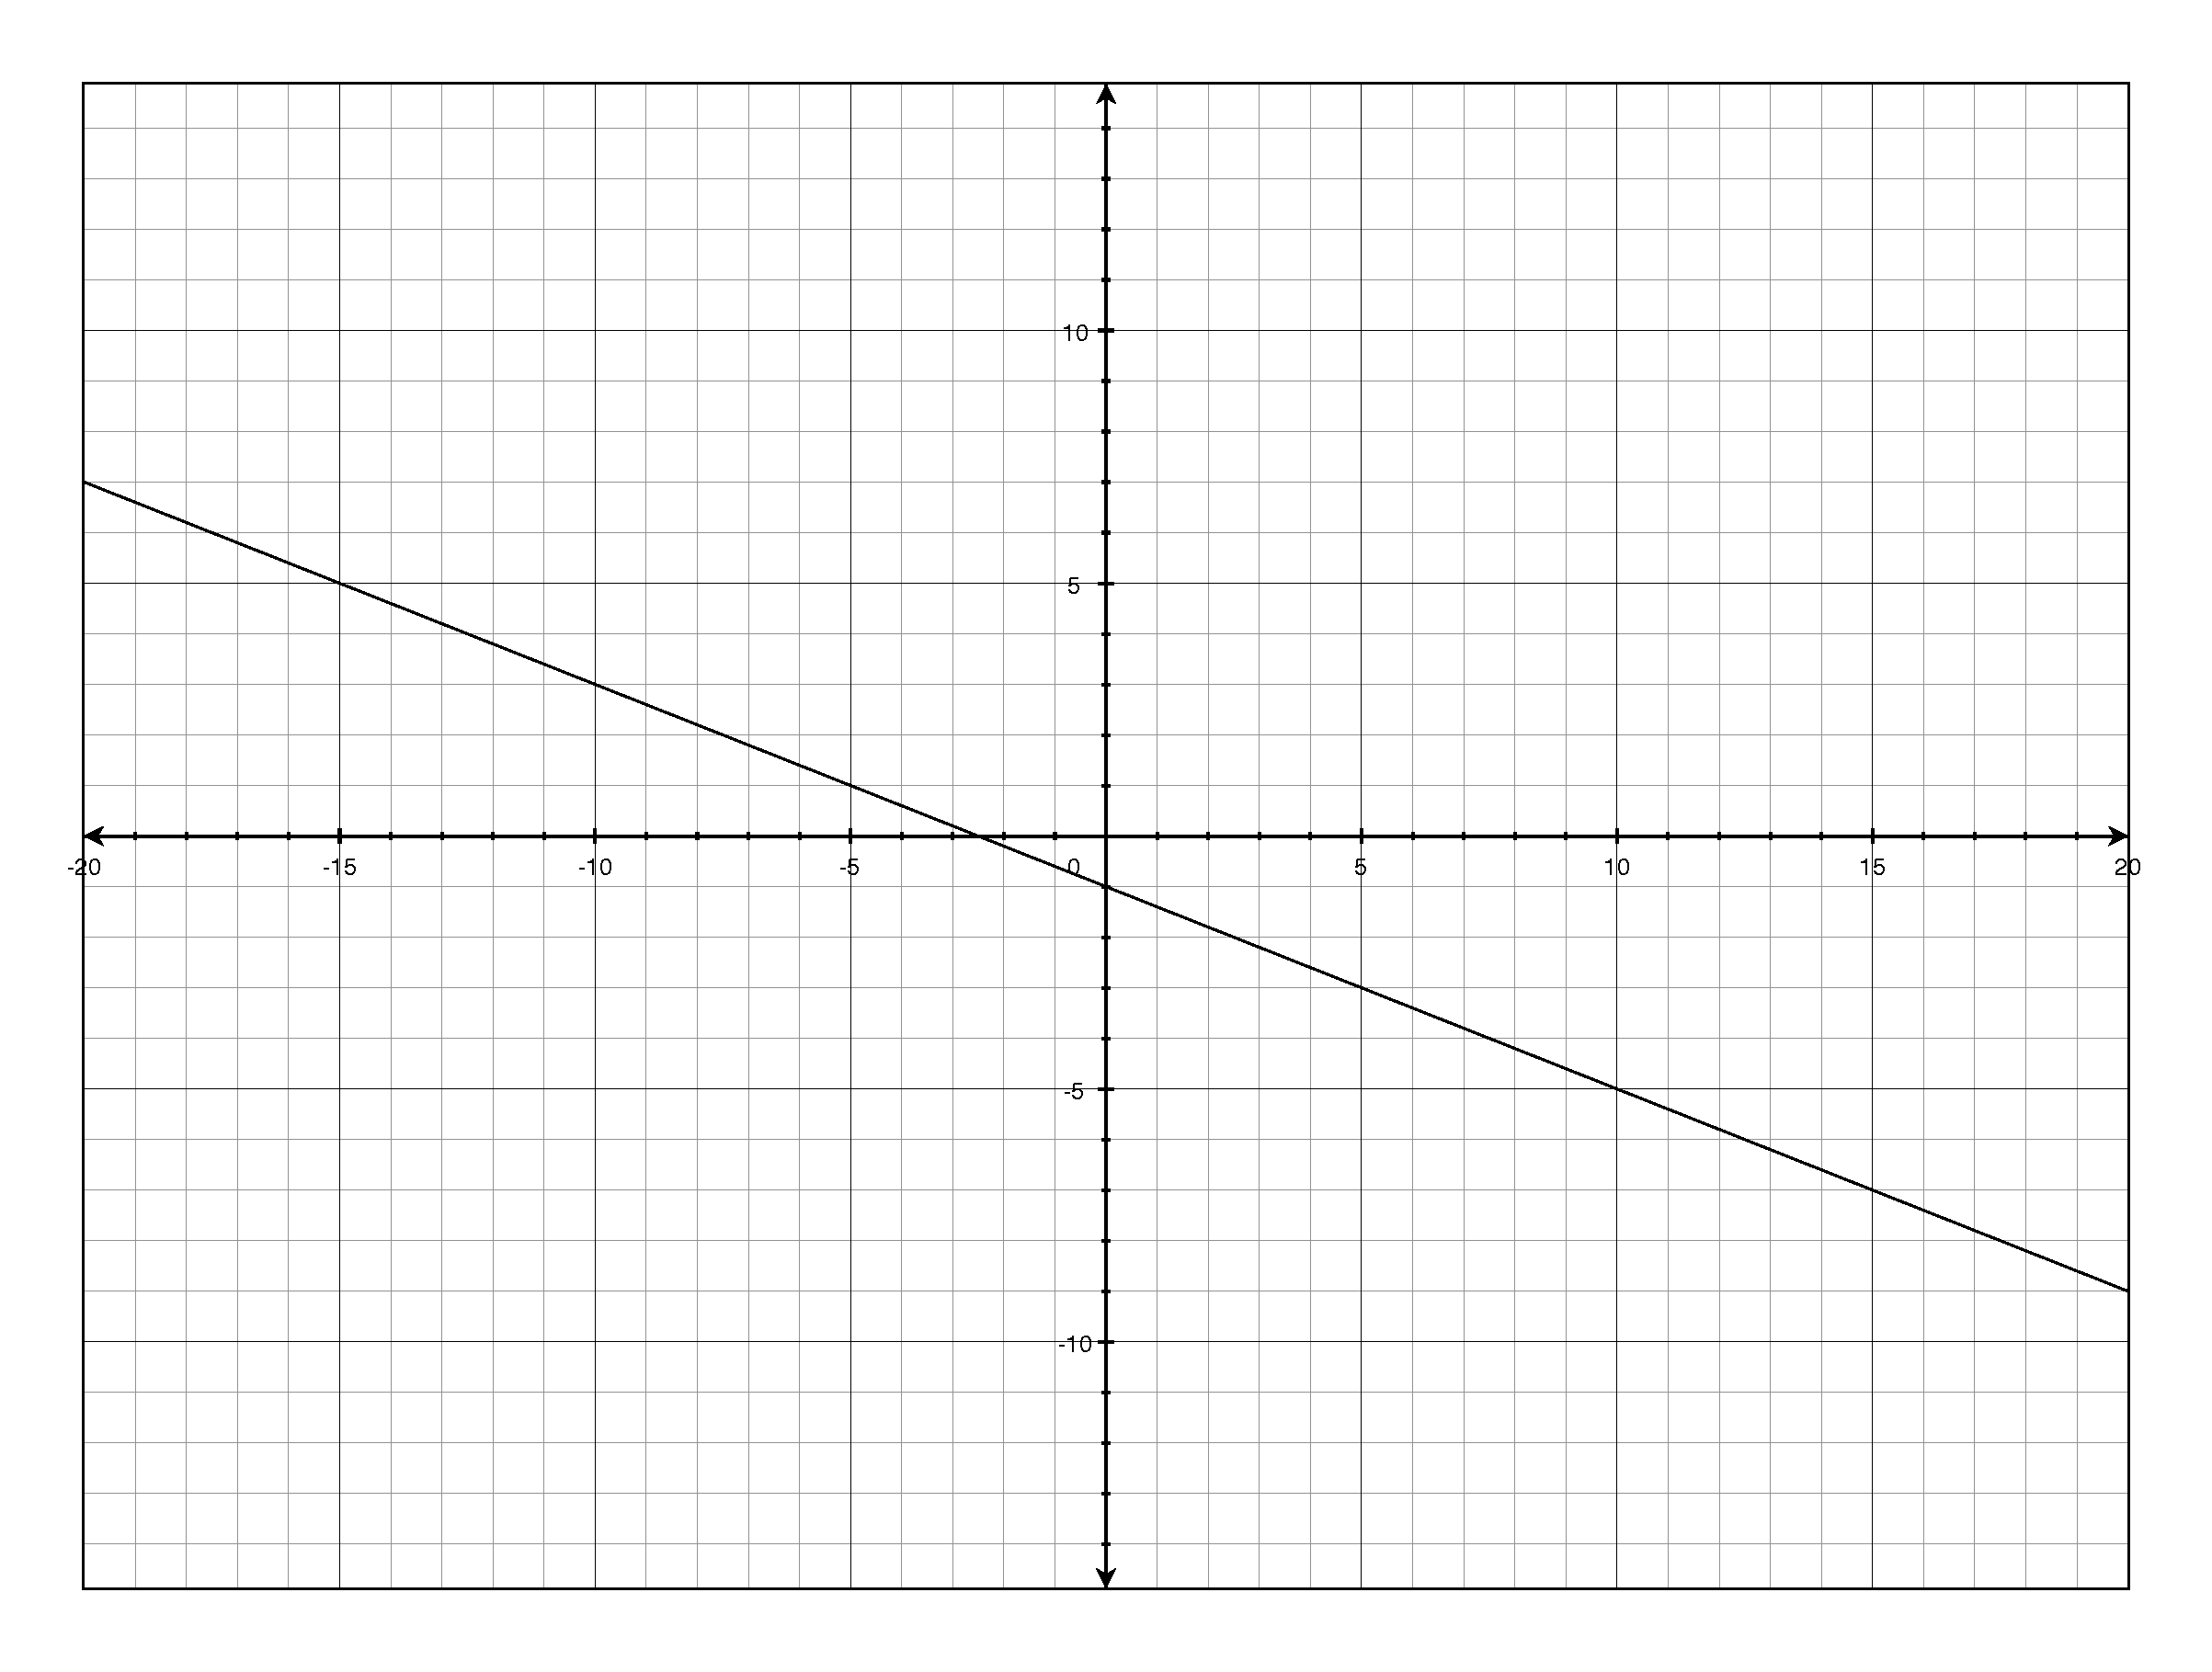
\includegraphics[width=9cm,height=7cm]{p386/57}
\end{figure}

\item[58]
$y = - \dfrac{1}{2} x + 3$

\begin{figure}[H]
  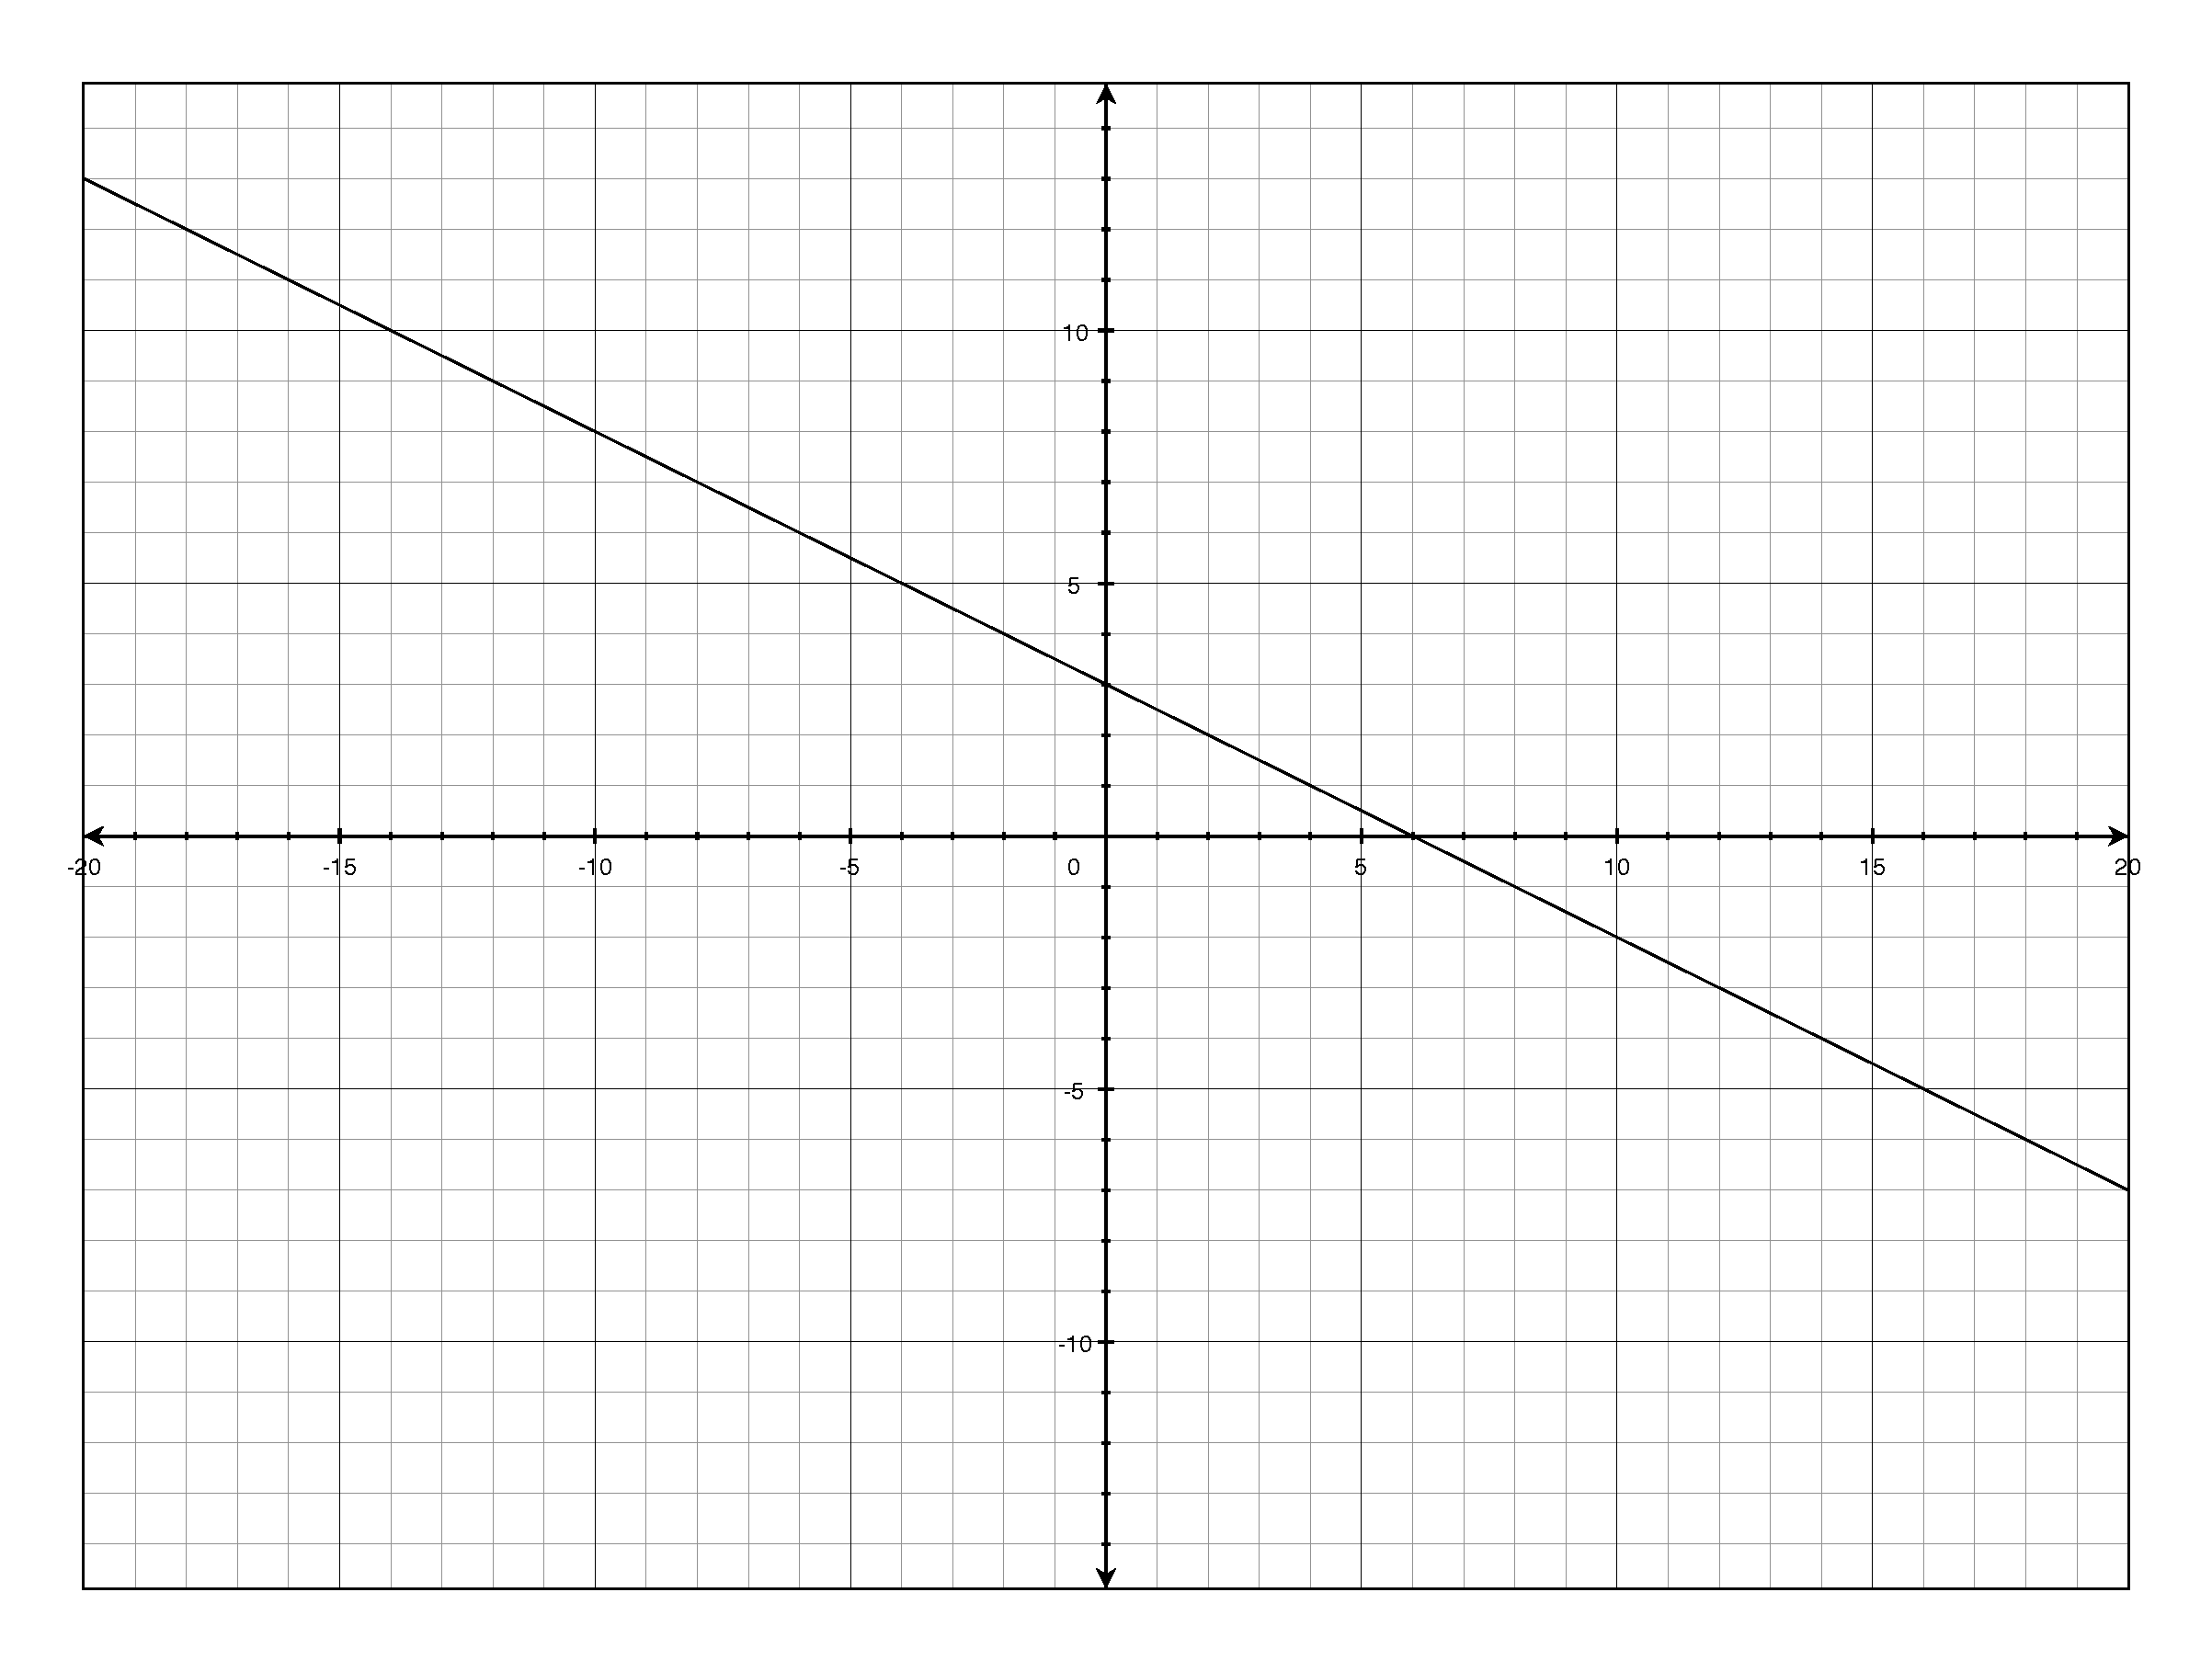
\includegraphics[width=9cm,height=7cm]{p386/58}
\end{figure}

\end{description}

\fi

\section{Review Problems}

%% Rico had the good idea of including some review problems on each of the remaining homework assignments to
%% help everyone prepare for the final.  So here they are.  
 
\begin{questions}
\question 
Solve:
\[ 
  12x - 3 = 7x+ 27 
\]

\begin{solution}
\begin{align*}
  12x - 3 &= 7x+ 27 \\
  5x - 3 &= 27 \\
  5x  &= 30 \\
  x &= 6
\end{align*}
\end{solution}

\question
Solve:
\[ 
  \frac{5x + 1}{3} + \frac{3x - 2}{6} = -\frac{2}{3} 
\]

\begin{solution}
\begin{align*}
  \frac{5x + 1}{3} + \frac{3x - 2}{6} &= -\frac{2}{3} \\
  \frac{2(5x + 1)}{6} + \frac{3x - 2}{6} &= -\frac{2}{3} \\
  \frac{10x + 2 + 3x - 2}{6} &= -\frac{2}{3} \\
  \frac{13x}{6} &= -\frac{2}{3} \\
  13x &= -\frac{12}{3} \\
  13x &= -4 \\
  x &= - \frac{4}{13} \\
\end{align*}

\end{solution}

\question
Solve:
\[ 
  12 - 3x \leq -13 
\]

\begin{solution}
\begin{align*}
  12 - 3x &\leq -13 \\
  -3x &\leq -25 \\
  x &\geq \frac{25}{3}
\end{align*}

$x = \left [ \dfrac{25}{3}, \infty \right) $

\end{solution}

\question
Solve:
\[ 
  |8x-3| \geq 13  
\]

\begin{solution}
\begin{eqnarray*}
  8x-3 \leq -13 & or & 8x-3 \geq 13 \\
  8x \leq -10 & or & 8x \geq 16 \\
  x \leq \frac{-10}{8} & or & x \geq \frac{16}{8} \\
  x \leq - \frac{5}{4} & or & x \geq 2 \\
\end{eqnarray*}

$x = \left( -\infty, -\dfrac{5}{4} \right] \cup [2, \infty)$

\end{solution}


\question
Simplify:
\[ 
  (2x - 1) + (7x + 3) - 4(5x + 4) 
\]

\begin{solution}
\[
  (2x - 1) + (7x + 3) - 4(5x + 4) = 9x+2 -20x-16 = -11x-14
\]
\end{solution}

\question
Factor:
\[
  x^2 + 4x - 21
\]

\begin{solution}
\[
  x^2 + 4x - 21 = (x+7)(x-3)
\]
\end{solution}

\question
Factor:
\[
  3x^2 + 7x - 6
\]

\begin{solution}
\[
  3x^2 + 7x - 6 = (3x - 2)(x + 3)
\]
\end{solution}

\question
Solve by factoring:
\[
  6x^2 - 11x + 4 = 0
\]

\begin{solution}
\begin{align*}
  6x^2 - 11x + 4 &= 0 \\
  (3x-4)(2x-1) &= 0 \\
  x &= \left \{ \frac{1}{2}, \frac{4}{3} \right \} \\
\end{align*}

check:
\begin{itemize}
  \item \( \dfrac{1}{2} + \dfrac{4}{3} = \dfrac{11}{6}  \)
  \item \( \dfrac{1}{2} \cdot \dfrac{4}{3} = \dfrac{4}{6} \)
\end{itemize}

\end{solution}

\question
Solve by factoring:
\[
  4x^2 - 20x + 25 = 0
\]

\begin{solution}
\begin{align*}
  4x^2 - 20x + 25 &= 0 \\
  (2x - 5)(2x-5) &= 0 \\
  x &= \frac{5}{2} \\
\end{align*}
check:
\begin{itemize}
  \item \( \dfrac{5}{2} + \dfrac{5}{2} = 5 \)
  \item \( \dfrac{5}{2} \cdot \dfrac{5}{2} = \dfrac{25}{4} \)
\end{itemize}

\end{solution}

\question
Simplify:
\[
  (3^{-1} + 2^{-3})^{-2}
\]

\begin{solution}
\begin{align*}
  (3^{-1} + 2^{-3})^{-2} &= \left( \frac{1}{3} + \frac{1}{8} \right)^{-2} \\
   &= \left( \frac{11}{24} \right)^{-2} \\
   &= \left( \frac{24}{11} \right)^{2} \\
   &= \frac{576}{121} \\
\end{align*}

\end{solution}

\question
Multiply and simplify:
\[
  \frac{4x^2}{5} \cdot \frac{15}{12x^2}
\]

\begin{solution}
\[
  \frac{4x^2}{5} \cdot \frac{15}{12x^2} = \frac{1}{x}
\]
\end{solution}

\question
Simplify:
\[
  \frac{2-x}{3x-6}
\]

\begin{solution}
\[
  \frac{2-x}{3x-6} = \frac{\cancel{(2-x)}} {-3 \cancel{(2-x)}} = - \frac{1}{3}
\]
\end{solution}

\question
Multiply and simplify:
\[
  \left( \frac{y^2 + 8y + 16}{2(y-2)} \right) \left( \frac{8y-16}{(y+4)^3} \right)
\]

\begin{solution}
  
\begin{align*}
  \left( \frac{y^2 + 8y + 16}{2(y-2)} \right) \left( \frac{8y-16}{(y+4)^3} \right)
  &= \left( \frac{(y+4)^2}{2 \cancel{(y-2)}} \right) \left( \frac{8 \cancel{(y-2)}} {(y+4)^3} \right) \\
  &= \frac{4(y+4)^2}{(y+4)^3} \\
  &= \frac{4}{y+4} \\
\end{align*}

\end{solution}

\question
Simplify:
\[
  \frac{\left( \cfrac{3x}{x+2} \right)}{\left( \cfrac{12}{x^3 + 2x^2} \right)}
\]

\begin{solution}
\begin{align*}
  \frac{\left( \cfrac{3x}{x+2} \right)}{\left( \cfrac{12}{x^3 + 2x^2} \right)}
  &= \frac{3x}{x+2} \cdot \frac{x^3 + 2x^2}{12} \\
  &= \frac{x \cdot x^2 \cancel{(x+2)} }{4 \cancel{(x+2)}} \\
  &= \frac{x^3}{4} \\
\end{align*}
\end{solution}

\question
Solve:
\[
  \frac{2}{x+5} - \frac{3}{x+3} = \frac{1}{x}
\]

\begin{solution}
\begin{align*}
  \frac{2}{x+5} - \frac{3}{x+3} &= \frac{1}{x} \\
  \frac{2x+6-3x-15}{(x+3)(x+5)} &= \frac{1}{x} \\
  \frac{-x-9}{x^2+8x+15} &= \frac{1}{x} \\
  x(-x-9) &= x^2+8x+15 \\
  -x^2-9x &= x^2+8x+15 \\
  2x^2 + 17x + 15 &= 0 \\
  (2x+15)(x+1) &= 0 \\
  x &= \left \{ -\frac{15}{2}, -1 \right \} \\
\end{align*}
\end{solution}

\end{questions}

\ifprintanswers
\else
\vspace{1.5 in}

\begin{em}
I do not know how I may appear to the world, but to myself I seem to have been only like a boy, playing on the
sea-shore, and diverting myself, in now and then finding a smoother pebble or prettier shell than ordinary, whilst the
great ocean of truth lay all undiscovered before me.
\end{em}

\vspace{0.1 in}
\hspace{0.5 in} --Isaac Newton

\fi

\end{document}

